\subsection{Konzept Blau}

\subsubsection{Vereinzelung mittels rotierender Lochmaske}
\begin{wrapfigure}[26]{r}{10cm}
	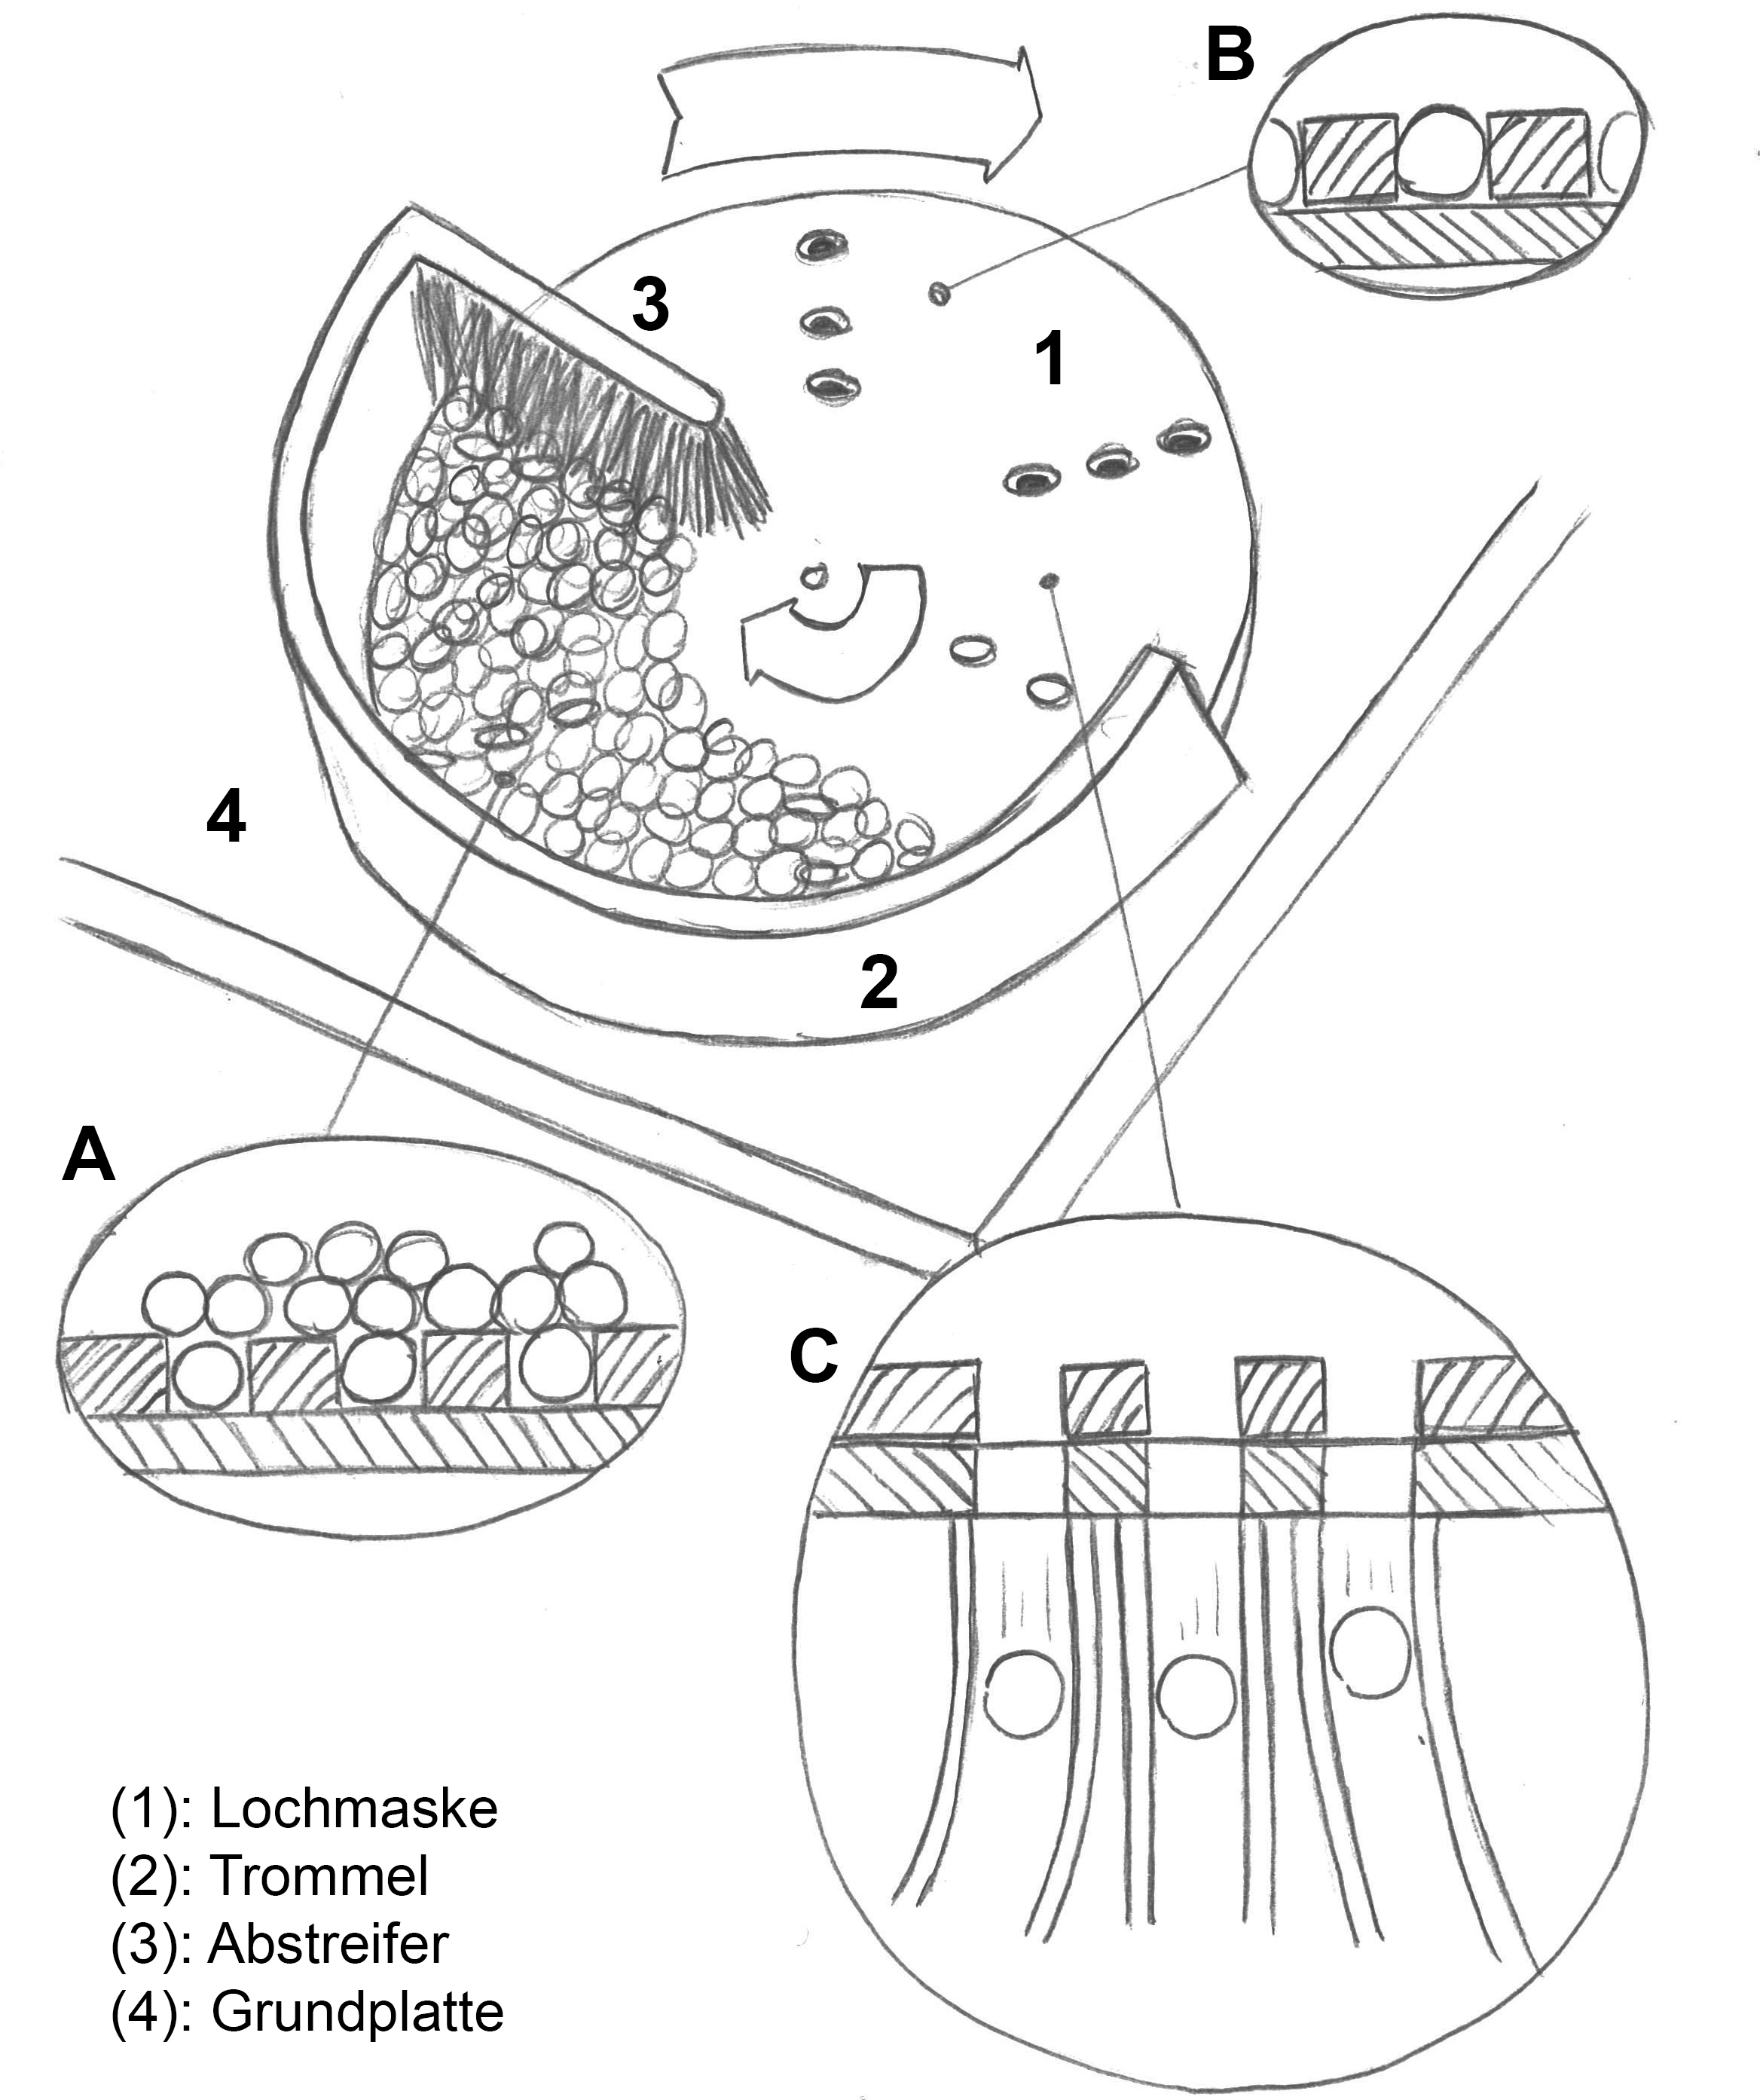
\includegraphics[scale=0.52]{Illustrationen/5-Konzept/schema_vereinzelung.jpg}
	\caption{Vereinzelung durch rotierende Lochmaske}
	\label{fig:schema_vereinzelung}
\end{wrapfigure}
Die Vereinzelung wird im Konzept  Blau durch eine rotierende Lochmaske realisiert. Die NemaCaps werden in einen Behälter gefüllt (Punkt 2 in Abbildung \ref{fig:schema_vereinzelung}). Darin befindet sich eine rotierend-gelagerte Scheibe mit Löchern (Lochmaske, 1). Die Öffnung ist so gestaltet, dass ein NemaCap hineinpasst. Durch die Rotation der Lochmaske fallen nun NemaCaps in die Löcher (Detail A) und werden zu Detail B transportiert. Ein Abstreifer (hier in Form einer Bürste) sorgt dafür, dass überschüssige NemaCaps zurückgehalten werden. In der Grundplatte (4) sind Löcher vorgesehen, welche die NemaCaps in Schläuche fallen lassen (Detail C). Idealerweise wird dieser Aufbau schief gelagert. 
\newline
Dieses Konzept wird von der Firma Kofatec GmbH erfolgreich für die Vereinzelung von Pfefferkörnern eingesetzt. 

\subsubsection{Setzen der NemaCaps durch Ausheben eines Setzloches}

\begin{figure}[H]
	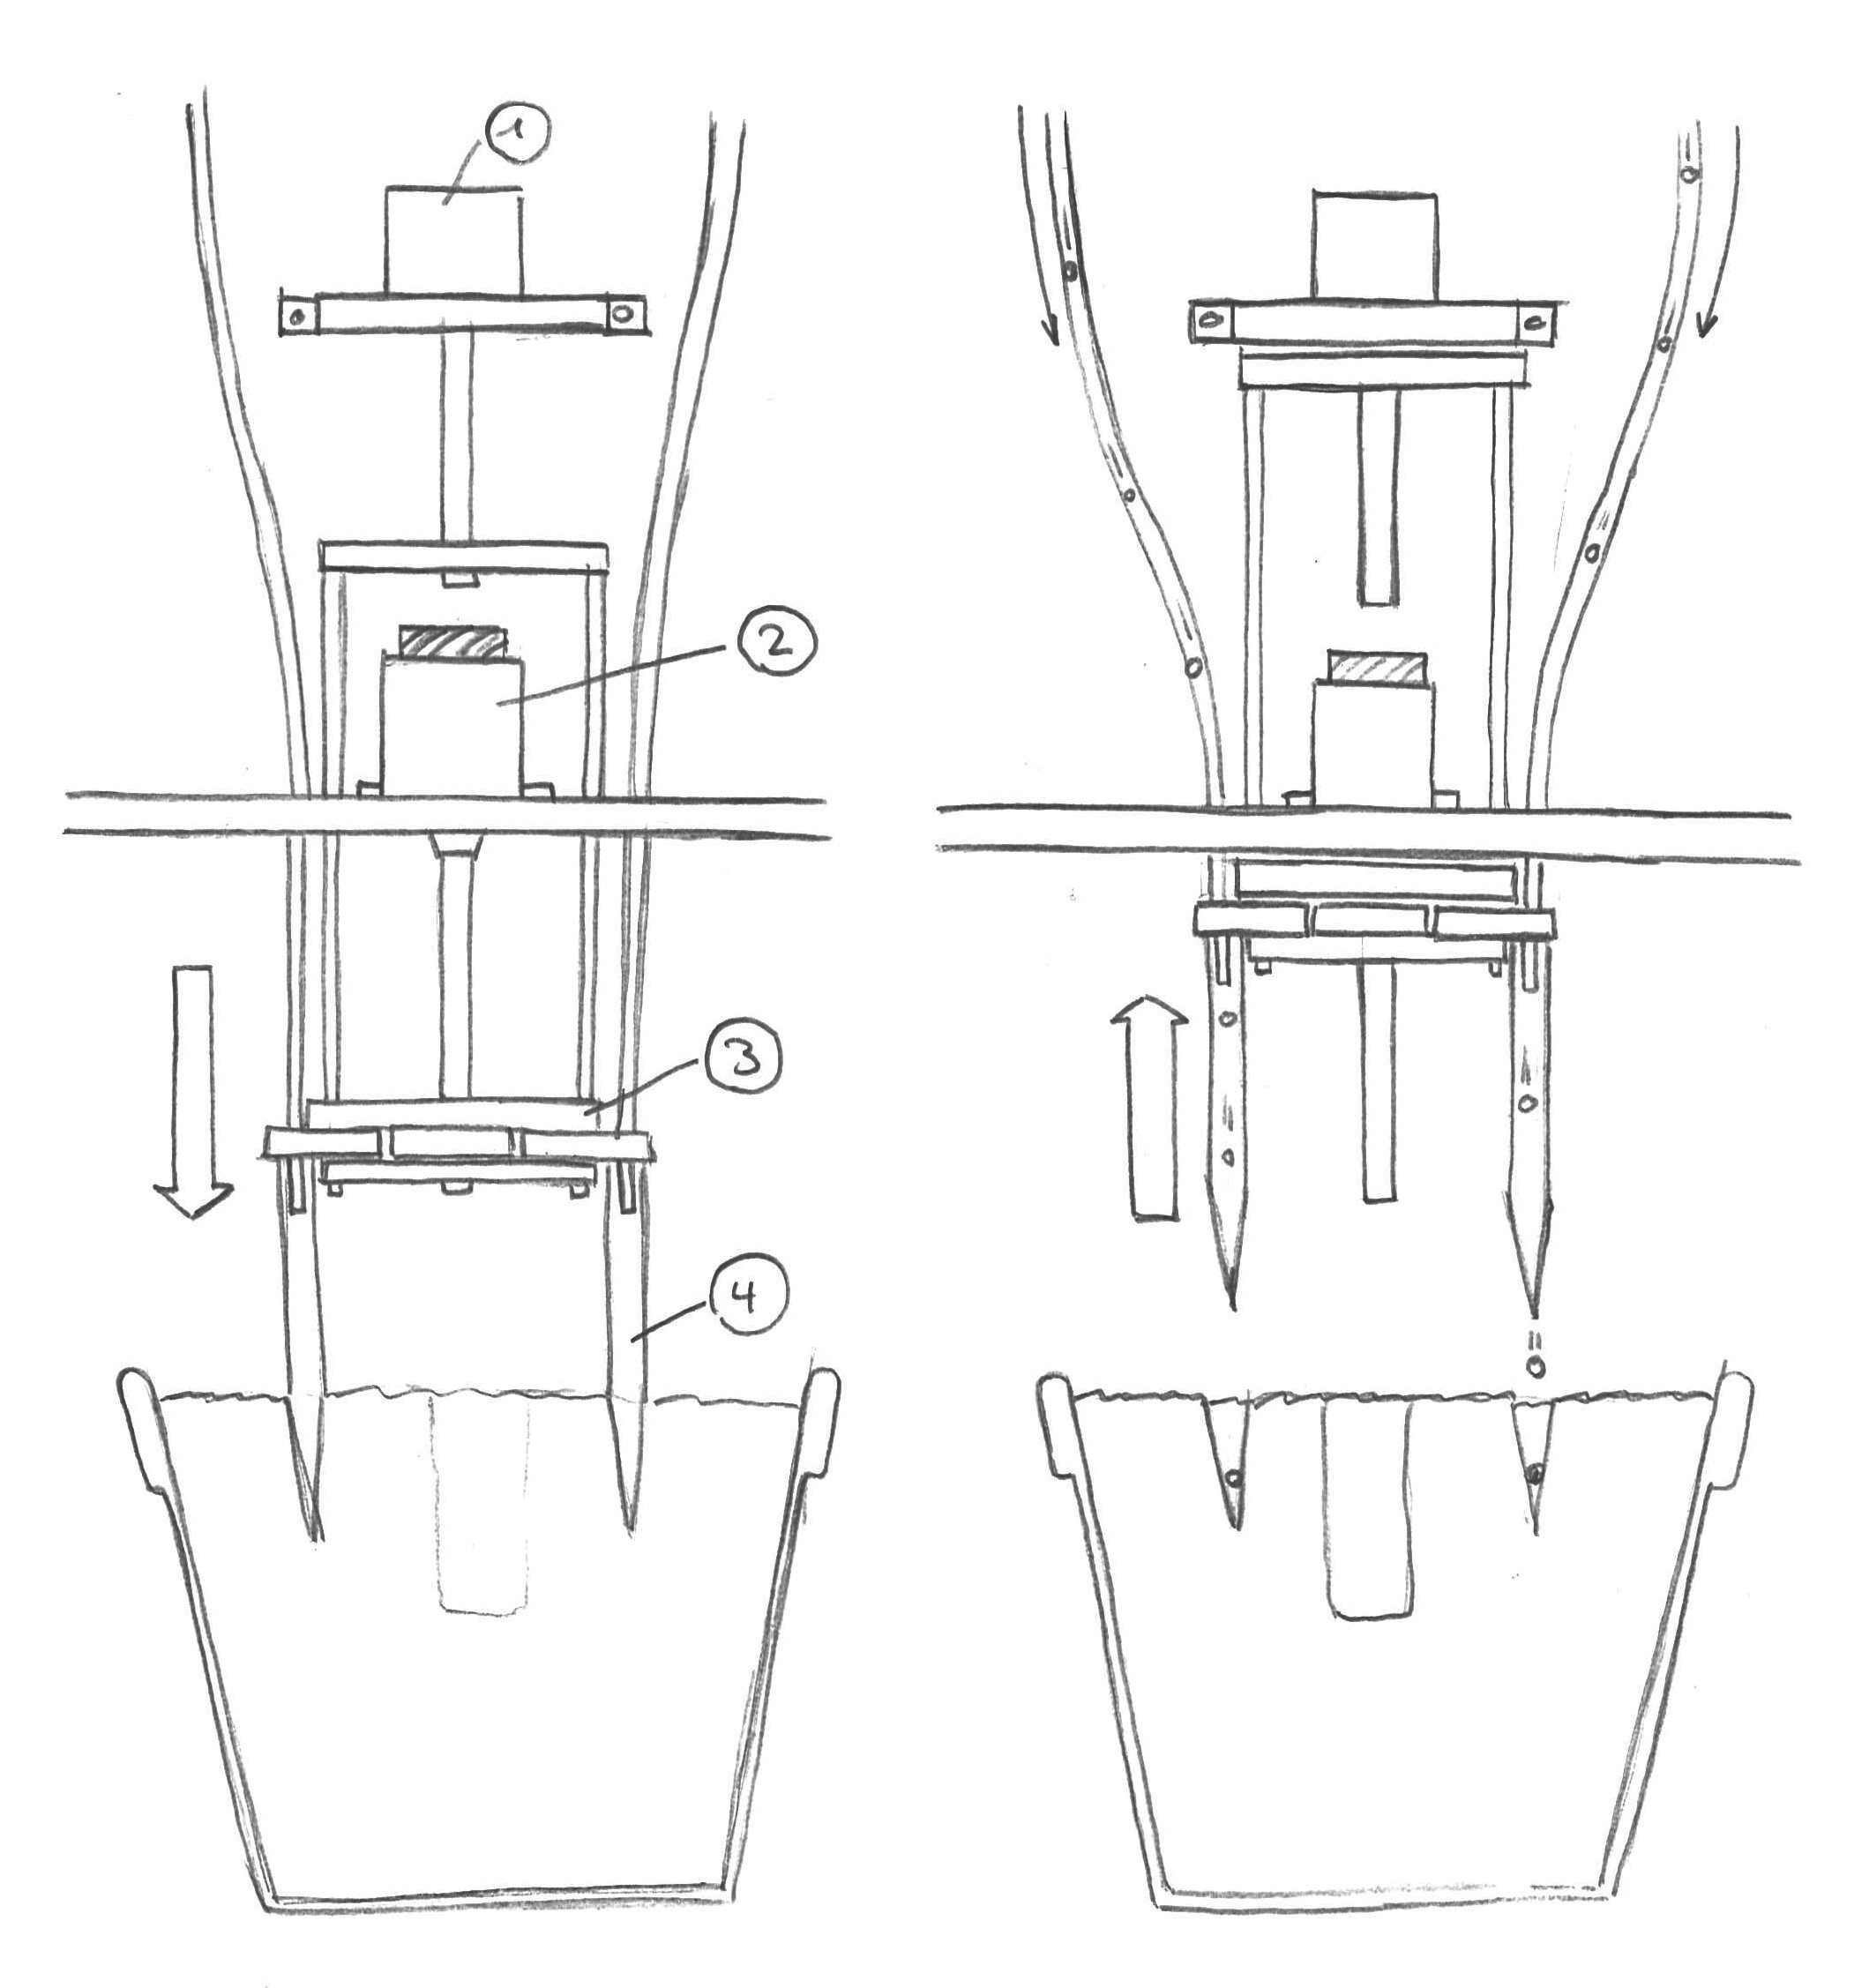
\includegraphics[width=1\textwidth]{Illustrationen/5-Konzept/blau_Setzeinheit_ohneLegende.jpg}
	\caption{Teilfunktionsmuster zur Vereinzelung der NemaCaps}
	\label{fig:blau_setzeinheit}
\end{figure}

\subsubsection{Setzmechanismus konfigurieren mittels Kulissen}

\begin{figure}[H]
	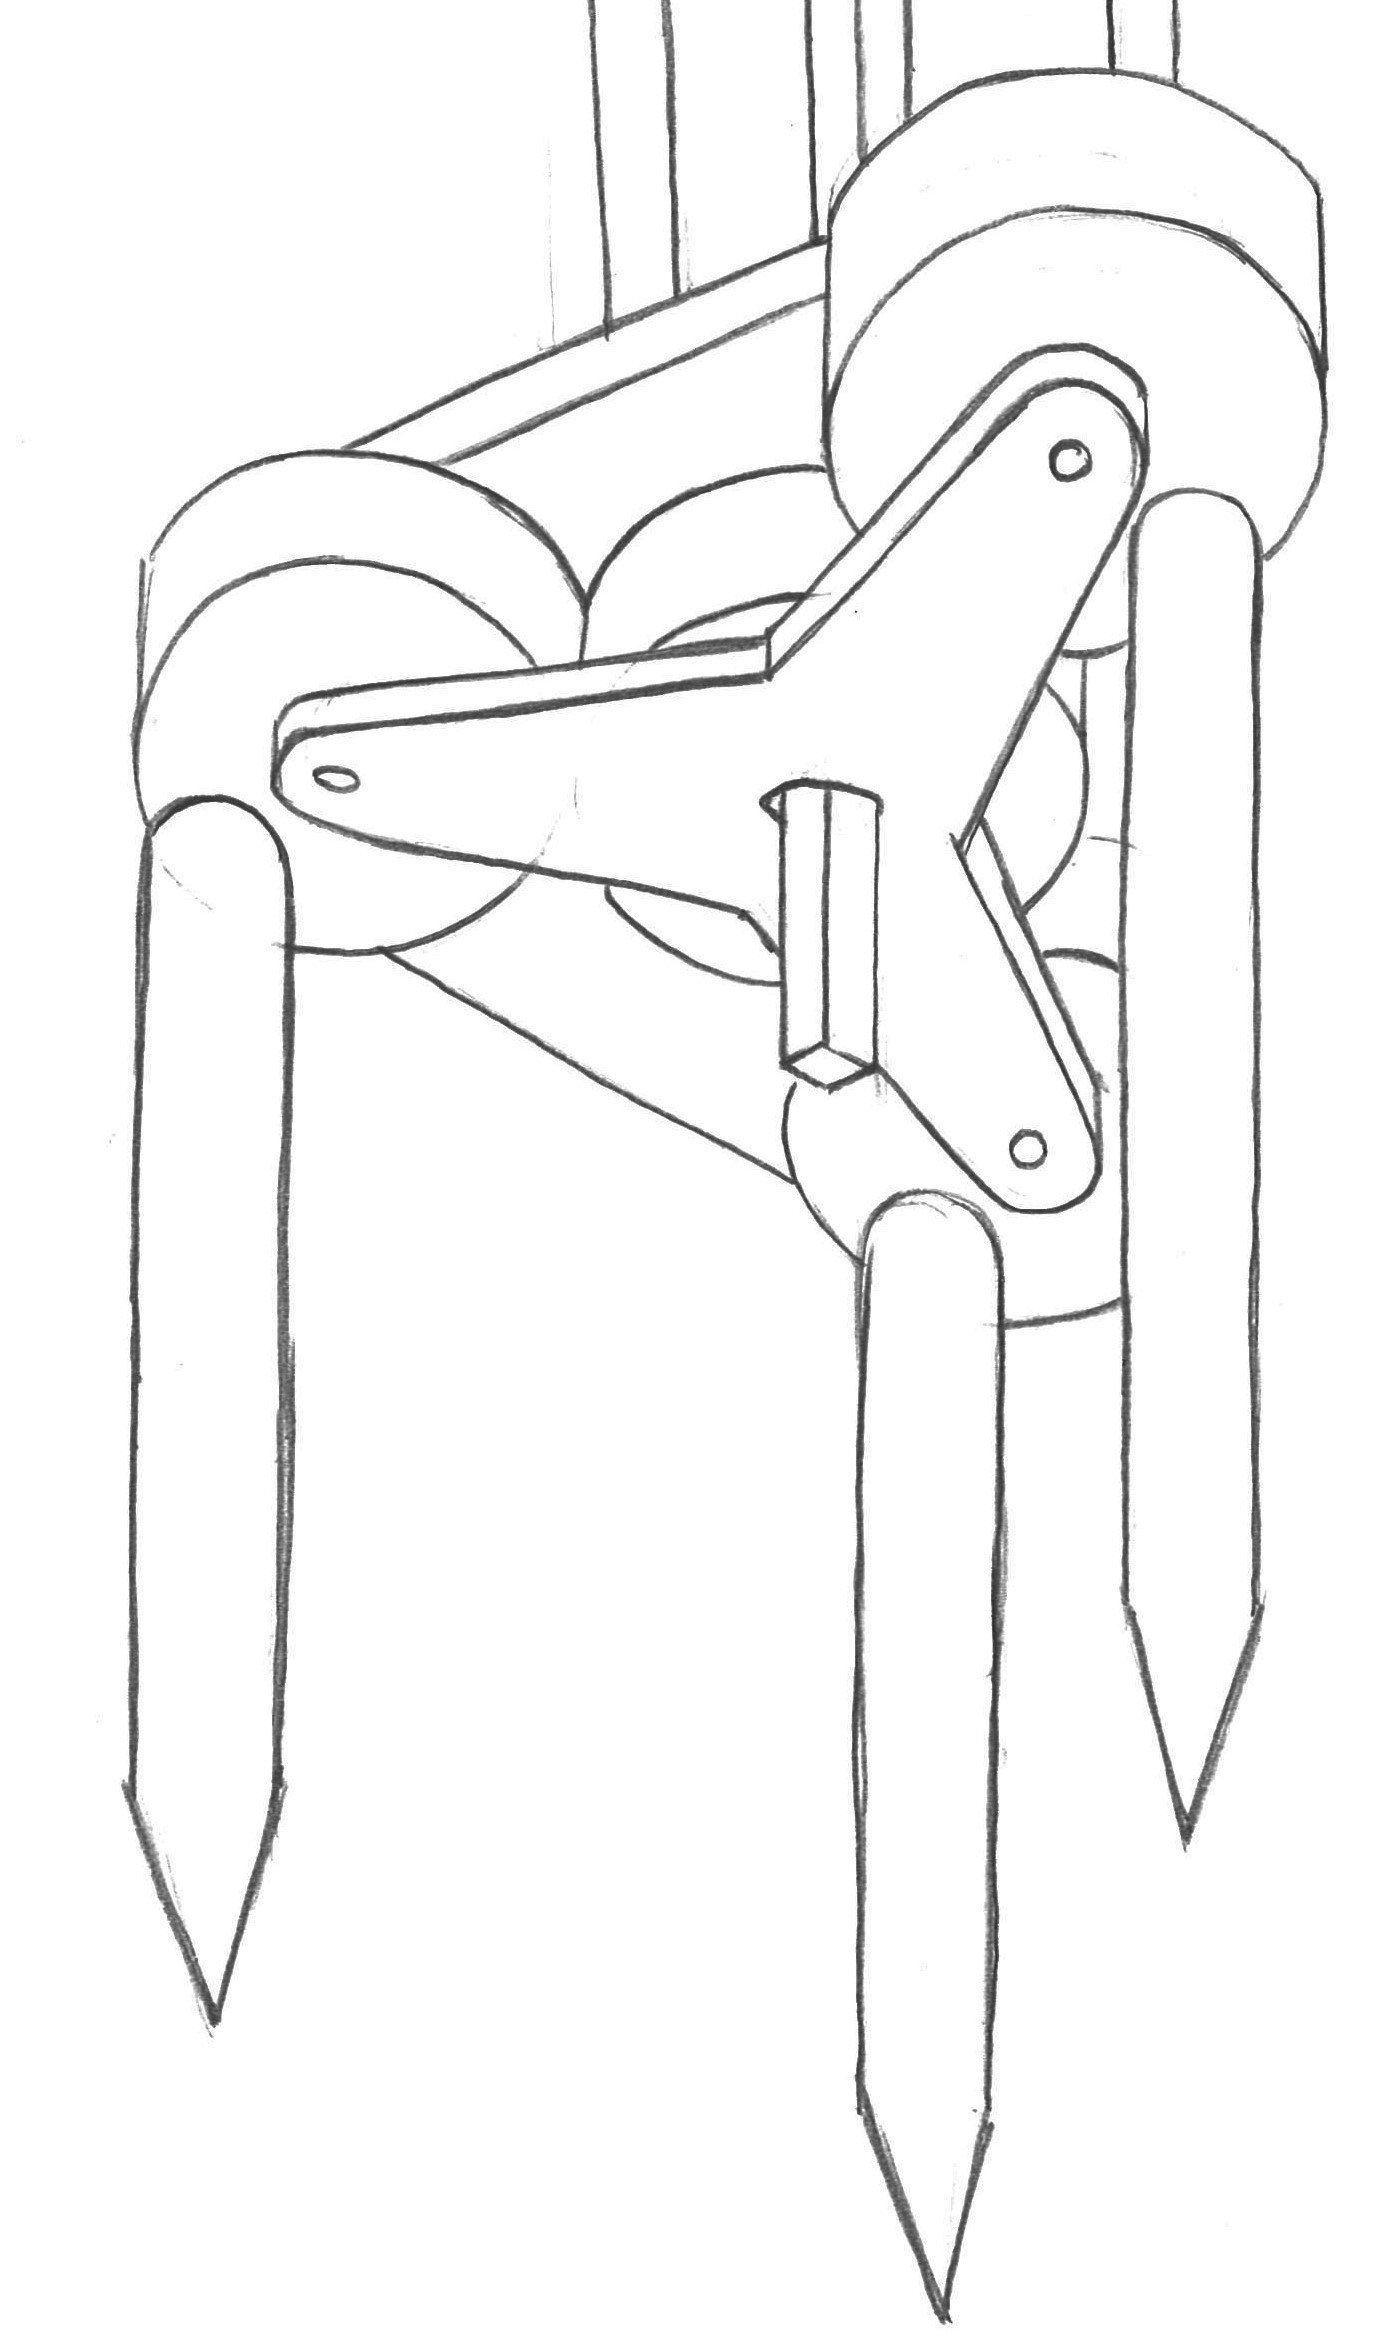
\includegraphics[scale=0.5]{Illustrationen/5-Konzept/blau_Verstellmechanismus.jpg}
	\caption{Teilfunktionsmuster zur Vereinzelung der NemaCaps}
	\label{fig:blau_verstellmech}
\end{figure}